\documentclass{standalone}
\usepackage{tikz}
\usetikzlibrary{patterns, positioning}

\begin{document}
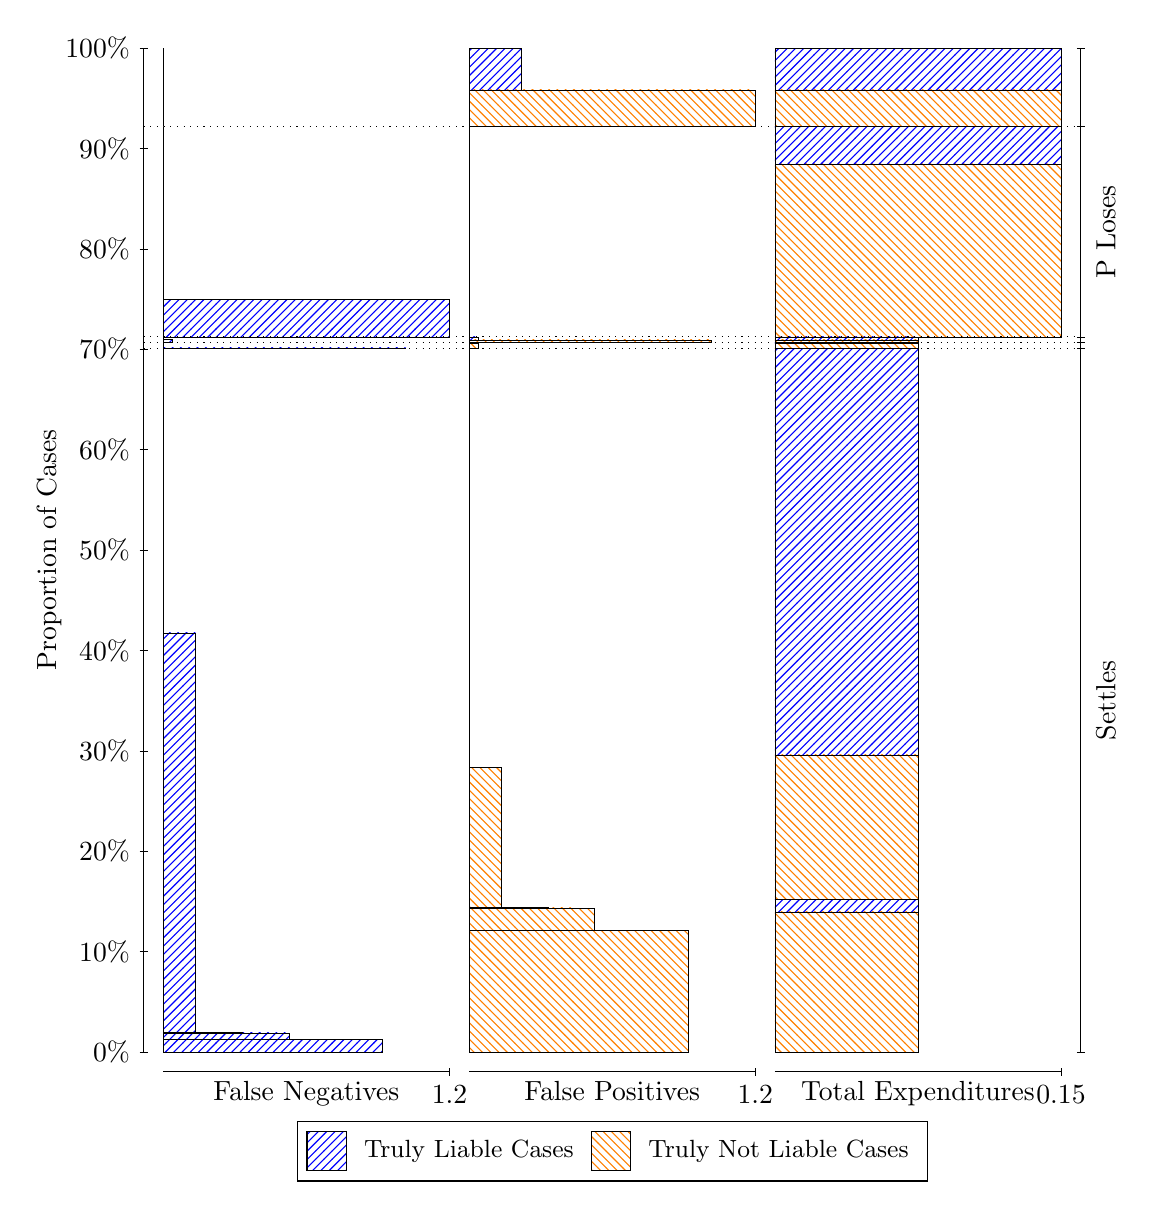
\begin{tikzpicture}
\draw[black, very thin] (1.5,1.75) -- (1.5,14.5);
\node[rotate=90, anchor=center] at (0.3, 8.125) {Proportion of Cases};
\draw[black, very thin] (1.45,1.75) -- (1.55,1.75);
\node[anchor=east] at (1.45, 1.75) {0\%};
\draw[black, very thin] (1.45,3.025) -- (1.55,3.025);
\node[anchor=east] at (1.45, 3.025) {10\%};
\draw[black, very thin] (1.45,4.3) -- (1.55,4.3);
\node[anchor=east] at (1.45, 4.3) {20\%};
\draw[black, very thin] (1.45,5.575) -- (1.55,5.575);
\node[anchor=east] at (1.45, 5.575) {30\%};
\draw[black, very thin] (1.45,6.85) -- (1.55,6.85);
\node[anchor=east] at (1.45, 6.85) {40\%};
\draw[black, very thin] (1.45,8.125) -- (1.55,8.125);
\node[anchor=east] at (1.45, 8.125) {50\%};
\draw[black, very thin] (1.45,9.4) -- (1.55,9.4);
\node[anchor=east] at (1.45, 9.4) {60\%};
\draw[black, very thin] (1.45,10.675) -- (1.55,10.675);
\node[anchor=east] at (1.45, 10.675) {70\%};
\draw[black, very thin] (1.45,11.95) -- (1.55,11.95);
\node[anchor=east] at (1.45, 11.95) {80\%};
\draw[black, very thin] (1.45,13.225) -- (1.55,13.225);
\node[anchor=east] at (1.45, 13.225) {90\%};
\draw[black, very thin] (1.45,14.5) -- (1.55,14.5);
\node[anchor=east] at (1.45, 14.5) {100\%};

\draw[black, very thin] (13.4,1.75) -- (13.4,14.5);
\draw[black, very thin] (13.35,1.75) -- (13.45,1.75);
\node[anchor=west] at (13.35, 1.75) {};
\draw[black, very thin] (13.35,10.684) -- (13.45,10.684);
\node[anchor=west] at (13.35, 10.684) {};
\draw[black, very thin] (13.35,10.762) -- (13.45,10.762);
\node[anchor=west] at (13.35, 10.762) {};
\draw[black, very thin] (13.35,10.832) -- (13.45,10.832);
\node[anchor=west] at (13.35, 10.832) {};
\draw[black, very thin] (13.35,13.501) -- (13.45,13.501);
\node[anchor=west] at (13.35, 13.501) {};
\draw[black, very thin] (13.35,14.5) -- (13.45,14.5);
\node[anchor=west] at (13.35, 14.5) {};

\draw[black, very thin, pattern color=blue, pattern=north east lines] (1.75,1.75) rectangle (4.5306,1.9104);
\draw[black, very thin, pattern color=blue, pattern=north east lines] (1.75,1.9104) rectangle (4.234,1.9109);
\draw[black, very thin, pattern color=blue, pattern=north east lines] (1.75,1.9109) rectangle (3.9374,1.9114);
\draw[black, very thin, pattern color=blue, pattern=north east lines] (1.75,1.9114) rectangle (3.6408,1.9119);
\draw[black, very thin, pattern color=blue, pattern=north east lines] (1.75,1.9119) rectangle (3.3442,1.993);
\draw[black, very thin, pattern color=blue, pattern=north east lines] (1.75,1.993) rectangle (3.0476,1.9936);
\draw[black, very thin, pattern color=blue, pattern=north east lines] (1.75,1.9936) rectangle (2.751,1.9941);
\draw[black, very thin, pattern color=blue, pattern=north east lines] (1.75,1.9941) rectangle (2.4544,1.9947);
\draw[black, very thin, pattern color=blue, pattern=north east lines] (1.75,1.9947) rectangle (2.1578,7.0714);
\draw[black, very thin, pattern color=orange, pattern=north west lines] (1.75,7.0714) rectangle (1.75,10.684);
\draw[black, very thin, pattern color=blue, pattern=north east lines] (1.75,10.684) rectangle (4.8272,10.692);
\draw[black, very thin, pattern color=orange, pattern=north west lines] (1.75,10.692) rectangle (1.75,10.762);
\draw[black, very thin, pattern color=blue, pattern=north east lines] (1.75,10.762) rectangle (1.8612,10.801);
\draw[black, very thin, pattern color=orange, pattern=north west lines] (1.75,10.801) rectangle (1.75,10.832);
\draw[black, very thin, pattern color=blue, pattern=north east lines] (1.75,10.832) rectangle (5.3833,11.305);
\draw[black, very thin, pattern color=orange, pattern=north west lines] (1.75,11.305) rectangle (1.75,13.501);
\draw[black, very thin, pattern color=orange, pattern=north west lines] (1.75,13.501) rectangle (1.75,13.967);
\draw[black, very thin, pattern color=blue, pattern=north east lines] (1.75,13.967) rectangle (1.75,14.5);
\draw[black, very thin, pattern color=orange, pattern=north west lines] (5.6333,1.75) rectangle (8.4139,3.2896);
\draw[black, very thin, pattern color=orange, pattern=north west lines] (5.6333,3.2896) rectangle (8.1173,3.2915);
\draw[black, very thin, pattern color=orange, pattern=north west lines] (5.6333,3.2915) rectangle (7.8207,3.2934);
\draw[black, very thin, pattern color=orange, pattern=north west lines] (5.6333,3.2934) rectangle (7.5241,3.2953);
\draw[black, very thin, pattern color=orange, pattern=north west lines] (5.6333,3.2953) rectangle (7.2276,3.5783);
\draw[black, very thin, pattern color=orange, pattern=north west lines] (5.6333,3.5783) rectangle (6.931,3.5783);
\draw[black, very thin, pattern color=orange, pattern=north west lines] (5.6333,3.5783) rectangle (6.931,3.5806);
\draw[black, very thin, pattern color=orange, pattern=north west lines] (5.6333,3.5806) rectangle (6.6344,3.5829);
\draw[black, very thin, pattern color=orange, pattern=north west lines] (5.6333,3.5829) rectangle (6.3378,3.5851);
\draw[black, very thin, pattern color=orange, pattern=north west lines] (5.6333,3.5851) rectangle (6.0412,5.3622);
\draw[black, very thin, pattern color=blue, pattern=north east lines] (5.6333,5.3622) rectangle (5.6333,10.684);
\draw[black, very thin, pattern color=orange, pattern=north west lines] (5.6333,10.684) rectangle (5.7446,10.753);
\draw[black, very thin, pattern color=blue, pattern=north east lines] (5.6333,10.753) rectangle (5.6333,10.762);
\draw[black, very thin, pattern color=orange, pattern=north west lines] (5.6333,10.762) rectangle (8.7105,10.793);
\draw[black, very thin, pattern color=blue, pattern=north east lines] (5.6333,10.793) rectangle (5.7446,10.832);
\draw[black, very thin, pattern color=orange, pattern=north west lines] (5.6333,10.832) rectangle (5.6333,13.028);
\draw[black, very thin, pattern color=blue, pattern=north east lines] (5.6333,13.028) rectangle (5.6333,13.501);
\draw[black, very thin, pattern color=orange, pattern=north west lines] (5.6333,13.501) rectangle (9.2667,13.967);
\draw[black, very thin, pattern color=blue, pattern=north east lines] (5.6333,13.967) rectangle (6.3007,14.5);
\draw[black, very thin, pattern color=orange, pattern=north west lines] (9.5167,1.75) rectangle (11.333,3.5293);
\draw[black, very thin, pattern color=blue, pattern=north east lines] (9.5167,3.5293) rectangle (11.333,3.6902);
\draw[black, very thin, pattern color=orange, pattern=north west lines] (9.5167,3.6902) rectangle (11.333,5.5231);
\draw[black, very thin, pattern color=blue, pattern=north east lines] (9.5167,5.5231) rectangle (11.333,10.684);
\draw[black, very thin, pattern color=orange, pattern=north west lines] (9.5167,10.684) rectangle (11.333,10.753);
\draw[black, very thin, pattern color=blue, pattern=north east lines] (9.5167,10.753) rectangle (11.333,10.762);
\draw[black, very thin, pattern color=orange, pattern=north west lines] (9.5167,10.762) rectangle (11.333,10.793);
\draw[black, very thin, pattern color=blue, pattern=north east lines] (9.5167,10.793) rectangle (11.333,10.832);
\draw[black, very thin, pattern color=orange, pattern=north west lines] (9.5167,10.832) rectangle (13.15,13.028);
\draw[black, very thin, pattern color=blue, pattern=north east lines] (9.5167,13.028) rectangle (13.15,13.501);
\draw[black, very thin, pattern color=orange, pattern=north west lines] (9.5167,13.501) rectangle (13.15,13.967);
\draw[black, very thin, pattern color=blue, pattern=north east lines] (9.5167,13.967) rectangle (13.15,14.5);
\draw[black, dotted] (1.5,10.684) -- (13.4,10.684);
\draw[black, dotted] (1.5,10.762) -- (13.4,10.762);
\draw[black, dotted] (1.5,10.832) -- (13.4,10.832);
\draw[black, dotted] (1.5,13.501) -- (13.4,13.501);
\draw[black, very thin] (1.75,1.5) -- (5.3833,1.5);
\node[anchor=north] at (3.5667, 1.5) {False Negatives};
\draw[black, very thin] (5.3833,1.45) -- (5.3833,1.55);
\node[anchor=north] at (5.3833, 1.45) {1.2};

\draw[black, very thin] (5.6333,1.5) -- (9.2667,1.5);
\node[anchor=north] at (7.45, 1.5) {False Positives};
\draw[black, very thin] (9.2667,1.45) -- (9.2667,1.55);
\node[anchor=north] at (9.2667, 1.45) {1.2};

\draw[black, very thin] (9.5167,1.5) -- (13.15,1.5);
\node[anchor=north] at (11.333, 1.5) {Total Expenditures};
\draw[black, very thin] (13.15,1.45) -- (13.15,1.55);
\node[anchor=north] at (13.15, 1.45) {0.15};

\node[black, centered, rotate=90] at (13.72, 6.2168) {Settles};


\node[black, centered, rotate=90] at (13.72, 12.167) {P Loses};


\draw (7.449999999999999,1.5) node[draw=none] (baseCoordinate) {};
\begin{scope}[align=center]
        \matrix[scale=0.5, draw=black, below=0.5cm of baseCoordinate, nodes={draw}, column sep=0.1cm]{
            \node[rectangle, draw, minimum width=0.5cm, minimum height=0.5cm, pattern=north east lines, pattern color=blue] {}; &
            \node[draw=none, font=\small] (B) {Truly Liable Cases}; &
            \node[rectangle, draw, minimum width=0.5cm, minimum height=0.5cm, pattern=north west lines, pattern color=orange] {}; &
            \node[draw=none, font=\small] (B) {Truly Not Liable Cases}; \\
            };
\end{scope}

\end{tikzpicture}
\end{document}